\documentclass[titlepage,a4paper,12pt,norsk]{IMFeksamen}
%\geometry{left=3.5cm,right=3.5cm,bottom=2cm}
\usepackage[utf8]{inputenc}
\trykkinfo[tosidig,sorthvit]
\emnekode{TMA4110}
\emnenavn{Matematikk 3 -- EKSEMPEL~2}
\eksamensdato{Når du vil}
\eksamenstid{Fire timer}
\fagligkontaktinfo{Spør på mattelab hvis du lurer på noe}{Nei}
\hjelpemiddel{Ingen trykte eller håndskrevne hjelpemidler tillatt.
 Bestemt, enkel kalkulator tillatt.
 (Casio fx-82ES PLUS, Casio fx-82EX,
  Citizen SR-270X, Citizen SR-270X College,
  Hewlett Packard HP30S)}
\anneninfo{Eksamenen består av ti oppgaver
Hver av disse teller like mye.
Alle svar må begrunnes.

\textbf{Merk.}
Dette er ikke en virkelig eksamen, men et eksempel for å vise
hvordan en eksamen kan se ut.
Hvis du ikke har nok godkjente øvinger, kan du levere svar på disse
oppgavene som en ekstra øving.
}
\runninghead{TMA4110 -- Eksamen høsten 2018 -- EKSEMPEL~2}
\usepackage[T1]{fontenc}
\usepackage{lmodern,amsmath,amssymb,amsfonts}
\usepackage{mathrsfs}
\usepackage{systeme}
\usepackage{tikz}

\newcommand{\N}{\mathbb{N}}
\newcommand{\Z}{\mathbb{Z}}
\newcommand{\Q}{\mathbb{Q}}
\newcommand{\R}{\mathbb{R}}
\newcommand{\C}{\mathbb{C}}

\newcommand{\M}{\mathcal{M}} % vektorrom av matriser
\newcommand{\Cf}{\mathcal{C}} % vektorrom av kontinuerlige funksjoner
\renewcommand{\P}{\mathcal{P}} % vektorrom av polynomer
\newcommand{\B}{\mathscr{B}} % basis

\renewcommand{\Im}{\operatorname{Im}}
\renewcommand{\Re}{\operatorname{Re}}

\newcommand{\abs}[1]{|#1|}
\newcommand{\intersect}{\cap}
\newcommand{\union}{\cup}
\newcommand{\fcomp}{\circ}
\newcommand{\iso}{\cong}

\newcommand{\roweq}{\sim}
\DeclareMathOperator{\Sp}{Sp}
\DeclareMathOperator{\Null}{Null}
\DeclareMathOperator{\Col}{Col}
\DeclareMathOperator{\Row}{Row}
\DeclareMathOperator{\rank}{rank}
\DeclareMathOperator{\im}{im}
\DeclareMathOperator{\id}{id}
\DeclareMathOperator{\Hom}{Hom}
\newcommand{\tr}{^\top}
\newcommand{\koord}[2]{[\,{#1}\,]_{#2}} % koordinater mhp basis

\newcommand{\V}[1]{\mathbf{#1}}
\newcommand{\vv}[2]{\begin{bmatrix} #1 \\ #2 \end{bmatrix}}
\newcommand{\vvS}[2]{\left[ \begin{smallmatrix} #1 \\ #2 \end{smallmatrix} \right]}
\newcommand{\vvv}[3]{\begin{bmatrix} #1 \\ #2 \\ #3 \end{bmatrix}}
\newcommand{\vvvv}[4]{\begin{bmatrix} #1 \\ #2 \\ #3 \\ #4 \end{bmatrix}}
\newcommand{\vvvvv}[5]{\begin{bmatrix} #1 \\ #2 \\ #3 \\ #4 \\ #5 \end{bmatrix}}
\newcommand{\vn}[2]{\vvvv{#1_1}{#1_2}{\vdots}{#1_#2}}

\newcommand{\e}{\V{e}}
\renewcommand{\u}{\V{u}}
\renewcommand{\v}{\V{v}}
\newcommand{\w}{\V{w}}
\renewcommand{\b}{\V{b}}
\newcommand{\x}{\V{x}}
\newcommand{\0}{\V{0}}

\newenvironment{amatrix}[1]{% "augmented matrix"
  \left[\begin{array}{*{#1}{c}|c}
}{%
  \end{array}\right]
}



\begin{document}


\begin{oppgave}
Vi skriver linjene på formen $y=f(x)$:
\begin{align*}
	y &= \frac{1-x}{2}\\
	y &= \frac{2-3x}{4}\\
	y &= \frac{3-4x}{6}
\end{align*}

\begin{center}
	\begin{tikzpicture}
	\draw[->] (-3,0) -- (4.2,0) node[right] {$x$};
	\draw[->] (0,-2) -- (0,3.5) node[above] {$y$};
	\draw[scale=1,domain=-3:3,smooth,variable=\x] plot ({\x},{0.5-0.5*\x});
	\draw[scale=1,domain=-3:3,smooth,variable=\x] plot ({\x},{0.5-0.75*\x});
	\draw[scale=1,domain=-3:3,smooth,variable=\x] plot ({\x},{0.5-0.67*\x});
	\end{tikzpicture}
\end{center}

Alle linjene skjerer samme punkt på $y$-aksen; systemet har én løsning.
\end{oppgave}


\begin{oppgave}
Vi radreduserer $[A, I]$ som svarer til å løse likningene $A\x=\V{e}_i$ simultant: 
\begin{align*}
\begin{bmatrix}
1 & -2 & 3 & 1 & 0 & 0\\
2 & -4 & 7 & 0 & 1 & 0\\
1 & -1 & 3 & 0 & 0 & 1
\end{bmatrix}
&\sim
\begin{bmatrix}
1 & -2 & 3 & 1  & 0 & 0\\
0 & 0  & 1 & -2 & 1 & 0\\
0 & 1  & 0 & -1 & 0 & 1
\end{bmatrix}
\sim 
\begin{bmatrix}
1 & -2 & 3 & 1  & 0 & 0\\
0 & 1  & 0 & -1 & 0 & 1\\
0 & 0  & 1 & -2 & 1 & 0
\end{bmatrix}\\
&\sim
\begin{bmatrix}
1 & 0 & 3 & -1 & 0 & 2\\
0 & 1 & 0 & -1 & 0 & 1\\
0 & 0 & 1 & -2 & 1 & 0
\end{bmatrix}
\sim
\begin{bmatrix}
1 & 0 & 0 & 5  & -3 & 2\\
0 & 1 & 0 & -1 & 0  & 1\\
0 & 0 & 1 & -2 & 1  & 0
\end{bmatrix}.
\end{align*}
Dette gir
\[
A^{-1}=
\begin{bmatrix}
5  & -3 & 2\\
-1 & 0  & 1\\
-2 & 1  & 0
\end{bmatrix}.
\]

Løsningen er
\begin{align*}
A\x&=\vvv{1}{2}{3}\\
A^{-1}A\x&=A^{-1}\vvv{1}{2}{3}\\
I\x&=\begin{bmatrix}
5  & -3 & 2\\
-1 & 0  & 1\\
-2 & 1  & 0
\end{bmatrix}
\vvv{1}{2}{3}\\
\x&=\vvv{-3}{2}{0}.
\end{align*}
\end{oppgave}


\begin{oppgave}
Innfør $v=y'$. Nå kan vi skrive om likningen til 
\[
v'-3v=0.
\]
Vi har altså et system
\[
\systeme{
y'=v,
v'=3v
},
\]
som kan skrives 
\[
\V{y}'=\begin{bmatrix}
0 & 1\\
0 & 3
\end{bmatrix}\V{y}
\]
hvor $\V{y}=\vv{y}{v}$.

Vi finner egenverdiene til matrisen:

\[
\det \begin{bmatrix}
-\lambda & 1\\
0 & 3-\lambda
\end{bmatrix}=-\lambda(3-\lambda)
\]
Egenverdiene er $0$ og~$3$. 


$\lambda=0$: 
\[
A-0I=A=\begin{bmatrix}
0 & 1\\
0 & 3
\end{bmatrix}\sim
\begin{bmatrix}
0 & 1\\
0 & 0
\end{bmatrix}
\]
Likningen for egenrommet er derfor $x_2=0$, slik at \[
E_0=\{\vv{t}{0}|\;\; t\in \mathbb{R}\}=\Sp\vv{1}{0}.
\]

$\lambda=3$: Tilsvarende finner vi at 
\[
E_3=\Sp\vv{1}{3}.
\]

Vi setter inn i fromelen for generell løsning:
\[
\V{y} =c_1\vv{1}{0}+c_2\vv{1}{3}e^{3t}.
\]

Den ikkehomogene likningen 
\[
y''-3y'-2 = e^t.
\]
kan skrives
\[
y''-3y' = e^t+2.
\]

Vi har altså allerede funnet generell løsning til den tilhørende homogene ligningen: $\V{y}=\vv{y}{y'}$ slik at 
\[
y_h=c_1+c_2e^{3t}
\]
Det gjenstår kun å finne en partikulær løsning.

Prøv en løsning som ligner på $e^{3t}+2$: $y=ae^{3t}+b$. Regn ut 
\begin{align*}
y'&=3ae^{3t}\\
y''&=9ae^{3t}.
\end{align*}
Sett inn i likningen:
\[
e^{3t}+2=y''-3y'=9ae^{3t}-9ae^{3t}=0.
\]

Dette gir oss ingen informasjon om $a$ og~$b$. Derfor prøver vi å multiplisere forslaget vårt med $t$: $y=tae^{3t}+bt$. Regn ut
\begin{align*}
y'&=ae^{3t}+3ate^{3t}+b\\
y''&=6ae^{3t}+9ate^{3t}.
\end{align*}
Sett inn i likningen:
\[
e^{3t}+2=y''-3y'=6ae^{3t}+9ate^{3t}-3ae^{3t}-9ate^{3t}-3b=3ae^{3t}-3b.
\]
Dette gir $a=\frac{1}{3}$ og~$b=-\frac{2}{3}$, og vi har en partikulær løsning
\[
y_p=\frac{t}{3}e^{3t}-\frac{2t}{3}.
\]


Den generelle løsningen til den ikkehomogene likningen:
\[
y=y_h+y_p=c_1+c_2e^{3t}+\frac{t}{3}e^{3t}-\frac{2t}{3}.
\]

\end{oppgave}

\begin{oppgave}
Anta at $A$ er en $3 \times 3$-matrise med egenverdiene $2$, $5$ og $-5$.
Finn alle egenverdiene til hver av matrisene $3A$ og $A^2$.

Observasjon:
Hvis $\lambda$ er en egenverdi til $A$, og $\v$ er en tilhørende egenvektor, så ser vi at
\begin{align*}
(3A)\v&=3(A\v)=3(\lambda\v)=(3\lambda)\v\\
A^2\v&=A(A\v)=A(\lambda \v)=\lambda (A\v)=\lambda(\lambda)\v=\lambda^2 \v.
\end{align*}
Dette betyr at $3\lambda$ er en egenverdi til $3A$ og $\lambda^2$ er en egenverdi til $A^2$. 

Denne observasjonen gir oss dermed at $6$, $15$ og~$-15$ er egenverdier til $3A$; $4$ og~$25$ er egenverdier til $A^2$.

Påstand: Dette er alle egenverdiene til $3A$ og $A^2$.

$3A$: Vi har tre \emph{ulike} egenverdier: $6$, $15$ og~$-15$. Egenvektorer fra ulike egenrom er lineært uavhengige (fra teorien om egenvektorer). Derfor har vi tre lineært uavhengige egenvektorer fra de ulike egenrommene. Tre lineært uavhengige vektorer i $\mathbb{R}^3$ spenner automatisk. Dermed har vi en basis av egenvektorer (et basiselement fra hvert egenrom). Hver vektor i $\mathbb{R}^3$ kan altså skives som en (unik) lineærkombinasjon av tre egenvektorer tilhørende de tre egenverdiene. Men da vet vi at det ikke kan finnes egenvektorer i $\mathbb{R}^3$ tilhørende noen andre egenverdier av matrisen $3A$ (også fra teorien om egenvektorer).

$A^2$: Nå har vi bare to \emph{ulike} egenverdier fordi $(\pm 5)^2=25$. Første del av argumentasjonen ovenfor garanterer derfor bare at vi har to lineært uavhengige egenvektorer. Men observasjonen viser at alle egenvektorene tilhørende $5$ og~$-5$ -- betraktet som egenverdier til $A$ -- også er egenvektorer tilhørende $25$ -- betraktet som egenverdier til $A^2$. Siden egenvektorer tilhørende $5$ og~$-5$ er lineært uavhengige må egenrommet til $25$ minst være todimensjonalt. Vi kan altså finne to lineært uavhengige egenvektorer i egenrommet til $25$. Tilsammen med en egenvektor fra egenrommet til $4$ har vi dermed tre lineært uavhengige egenvektorer av $A^2$. Nå er resten av argumentasjonen helt lik som siste del av argumentasjonen for $3A$.

\emph{Merk}: Teorien som er brukt er oppsummert i Teorem \textbf{7.15.} fra forelesningsnotatene.
\end{oppgave}



\begin{oppgave}
Bruk minste kvadrats metode til å finne en approksimasjon til likningssystemet
\[
\systeme{
x + 2y = 1,
3x + 4y = 2,
5x + 6y = 3
}
\]
På matriseform:
\[
A\x=\b 
\]
hvor 
\[
A=\begin{bmatrix}
1 & 2\\
3 & 4\\
5 & 6
\end{bmatrix},\quad 
\b=\vvv{1}{2}{3}.
\]
Minste kvadraters metode: Løs likningen \[
A\tr A=A\tr \b.
\]

Vi regner ut 
\begin{align*}
A\tr A&= 
\begin{bmatrix}
1 & 3 & 5\\
2 & 4 & 6
\end{bmatrix}
\begin{bmatrix}
1 & 2\\
3 & 4\\
5 & 6
\end{bmatrix}=
\begin{bmatrix}
35 & 44\\
44 & 56 
\end{bmatrix}\\
A\tr \b&=
\begin{bmatrix}
1 & 3 & 5\\
2 & 4 & 6
\end{bmatrix} \vvv{1}{2}{3} =
\vv{22}{28}. 
\end{align*}

Radreduser totalmatrisen:
\begin{align*}
\begin{bmatrix}
35 & 44 & 22\\
44 & 56 & 28
\end{bmatrix}
&\sim
\begin{bmatrix}
1 & \frac{44}{35} & \frac{22}{35}\\
44 & 56 & 28
\end{bmatrix}\\
&\sim
\begin{bmatrix}
1 & \frac{44}{35} & \frac{22}{35}\\
0 & \frac{24}{35} & \frac{12}{35}
\end{bmatrix}\\
&\sim
\begin{bmatrix}
1 & \frac{44}{35} & \frac{22}{35}\\
0 & 2 & 1
\end{bmatrix}.
\end{align*}
Vi ser direkte at $x_2=\frac{1}{2}$. Innsatt i første likning får vi
\[
x_1+\frac{44}{35}\frac{1}{2}=\frac{22}{35}
\]
som gir $x_1=0$. Minste kvadraters løsning er derfor $\vv{0}{\frac{1}{2}}$.


Er dette en eksakt løsning?

\[
A\vv{0}{\frac{1}{2}}=\begin{bmatrix}
1 & 3 & 5\\
2 & 4 & 6
\end{bmatrix}\vv{0}{\frac{1}{2}}
=
\vvv{1}{2}{3}=\b.
\]
Ja.
\end{oppgave}


\begin{oppgave}
Den transponerte til rotasjonsmatrisen er
\[
\begin{bmatrix}
\cos \theta  & -\sin \theta  \\  \sin \theta & \cos \theta 
\end{bmatrix}\tr 
=
\begin{bmatrix}
\cos \theta  & \sin \theta  \\  -\sin \theta & \cos \theta 
\end{bmatrix}.
\]
Bruk at $\cos ^2 \theta +\sin^2 \theta =1$ for å regne ut
\begin{align*}
\begin{bmatrix}
\cos \theta  & -\sin \theta  \\  \sin \theta & \cos \theta 
\end{bmatrix}\tr 
\begin{bmatrix}
\cos \theta  & -\sin \theta  \\  \sin \theta & \cos \theta 
\end{bmatrix}
&=
\begin{bmatrix}
\cos^2 \theta +\sin^2 \theta   & -\cos\theta \sin \theta  +\cos\theta \sin \theta \\  
\cos\theta \sin \theta  -\cos\theta \sin \theta& \cos^2 \theta +\sin^2\theta
\end{bmatrix}\\
&=
\begin{bmatrix}
1 & 0 \\
0 & 1
\end{bmatrix}
=I.
\end{align*}
Derfor er rotasjonsmatrisen -- per definisjon -- ortogonal.

Matrisen $A$ beskrevet i oppgaveteksten tilfredstiller \[
A=VDV\tr
\]
hvor \[
V=\begin{bmatrix}
\cos \theta  & -\sin \theta  \\  \sin \theta & \cos \theta 
\end{bmatrix}, \quad
D=
\begin{bmatrix}
1 & 0 \\
0 & 2
\end{bmatrix},
\]
slik at 
\begin{align*}
A&=
\begin{bmatrix}
\cos \theta  & -\sin \theta  \\  \sin \theta & \cos \theta 
\end{bmatrix}
\begin{bmatrix}
1 & 0 \\
0 & 2
\end{bmatrix}
\begin{bmatrix}
\cos \theta  & \sin \theta  \\  -\sin \theta & \cos \theta 
\end{bmatrix}\\
&=
\begin{bmatrix}
\cos \theta  & -2\sin \theta  \\  \sin \theta & 2\cos \theta 
\end{bmatrix}
\begin{bmatrix}
\cos \theta  & \sin \theta  \\  -\sin \theta & \cos \theta 
\end{bmatrix}\\
&=
\begin{bmatrix}
\cos^2 \theta +2\sin^2 \theta   & \cos\theta \sin \theta  -2\cos\theta \sin \theta \\  
\cos\theta \sin \theta  -2\cos\theta \sin \theta& 2\cos^2 \theta +\sin^2\theta
\end{bmatrix}\\
&=
\begin{bmatrix}
1+\sin^2 \theta   & -\cos\theta \sin \theta \\  
-\cos\theta \sin \theta& 1+\cos^2 \theta
\end{bmatrix}.
\end{align*}

Når vi velger $\theta$ lik 45 grader får vi 
\[
V=
\begin{bmatrix}
\frac{1}{\sqrt{2}}  & -\frac{1}{\sqrt{2}}  \\ \frac{1}{\sqrt{2}} & \frac{1}{\sqrt{2}}
\end{bmatrix}, \quad
A= \begin{bmatrix}
\frac{3}{2}   & -\frac{1}{2}\\  
-\frac{1}{2}& \frac{3}{2}
\end{bmatrix}.
\]


Denne matrisen skalerer med en faktor $1$ langs $\vv{\frac{1}{\sqrt{2}}}{\frac{1}{\sqrt{2}}}$; en faktor $2$ langs $\vv{-\frac{1}{\sqrt{2}}}{\frac{1}{\sqrt{2}}}$. Derfor blir bildet av sirkelen en ellipse med halvakser av lengde $1$ langs den første egenvektoren og lengde $2$ langs den andre egenvektoren:

\begin{center}
	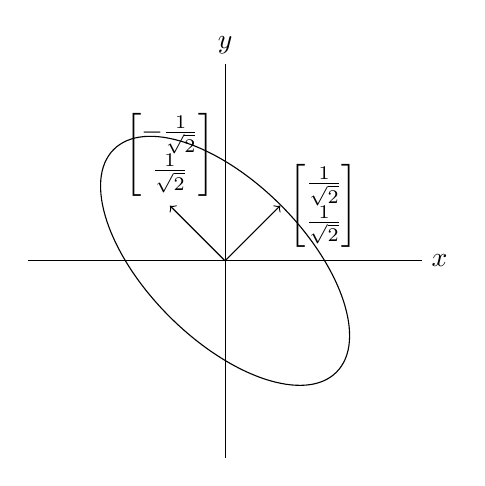
\begin{tikzpicture}
	\draw (-2.5,0) -- (2.5,0) node[right]{$x$};
	\draw (0,-2.5) -- (0,2.5) node[above]{$y$};
    \draw[->] (0,0) -- (0.7,0.7) node[right]{$\vv{\frac{1}{\sqrt{2}}}{\frac{1}{\sqrt{2}}}$};
    \draw[->] (0,0) -- (-0.7,0.7) node[above]{$\vv{-\frac{1}{\sqrt{2}}}{\frac{1}{\sqrt{2}}}$};
	\draw[rotate=45] (0,0) ellipse (1cm and 2cm);
	%\node at (1.1,0) [above] {$1$};
	%\node at (0,1.2) [left] {$1$};
	\end{tikzpicture}
\end{center}





\end{oppgave}


\begin{oppgave}
La $A$ være følgende matrise:
\[
A =
\begin{bmatrix}
-9 &  20 & -10 \\
 0 &   1 &   0 \\
 5 & -10 &   6
\end{bmatrix}
\]
Finn alle vektorer $\x$ slik at $A^2 \x = A \x$.
% \Sp \{ \vvv{2}{1}{0}, \vvv{-1}{0}{1} \}

Regn ut $A^2$:

\[
A^2=
\begin{bmatrix}
-9 &  20 & -10 \\
0 &   1 &   0 \\
5 & -10 &   6
\end{bmatrix}
\begin{bmatrix}
-9 &  20 & -10 \\
0 &   1 &   0 \\
5 & -10 &   6
\end{bmatrix}
=
\begin{bmatrix}
31 &  -60 & 30 \\
0 &   1 &   0 \\
-15 & 30 &   -14
\end{bmatrix}
\]

Skriv om: 
\begin{align*}
A^2\x&=A\x\\
A^2\x-A\x&=\0\\
(A^2-A)\x&=0
\end{align*}
Oppgaven er altså ekvivalent med å finne nullrommet til matrisen $A^2-A$:

\[
A^2-A=
\begin{bmatrix}
31 &  -60 & 30 \\
0 &   1 &   0 \\
-15 & 30 &   -14
\end{bmatrix}-
\begin{bmatrix}
-9 &  20 & -10 \\
0 &   1 &   0 \\
5 & -10 &   6
\end{bmatrix}
=
\begin{bmatrix}
40 &  -80 & 40 \\
0 &   0 &   0 \\
-20 & 40 &   -24
\end{bmatrix}.
\]
Som alltid radreduserer vi for å finne nullrommet:

\[
\begin{bmatrix}
40 &  -80 & 40 \\
0 &   0 &   0 \\
-20 & 40 &   -24
\end{bmatrix}
\sim
\begin{bmatrix}
1 &  -2 & 1 \\
0 &   0 &   0 \\
-1 & 2 &   -1
\end{bmatrix}
\sim
\begin{bmatrix}
1 &  -2 & 1 \\
0 &   0 &   0 \\
0 & 0 &   0
\end{bmatrix}
\]
Likningen for nullrommet er $x_1-2x_2+x_3=0$. Det er to frie variabler; vi kan for eksempel velge $x_2=t$ og $x_3=s$. Dette gir parametriseringen
\[
\{\vvv{2t-s}{t}{s}|\;\; t,s\in\mathbb{R}\}.
\]
\end{oppgave}



\begin{oppgave}
Husk at vi skriver $\P_2$ for vektorrommet som består av alle
polynomfunksjoner av grad~$2$ eller lavere.  La $p_1$, $p_2$, $p_3$
og~$q$ være følgende polynomer i~$\P_2$:
\begin{align*}
p_1(x) &= x^2 - 2    &   q(x) &= 4x^2 + x - 7  \\
p_2(x) &= -x^2 + x + 2 \\
p_3(x) &= 3x^2 + x - 5
\end{align*}
Vis at $\B = (p_1, p_2, p_3)$ er en basis for $\P_2$,
og finn koordinatene $[ q ]_\B$ til $q$ med hensyn på denne basisen.
\end{oppgave}


\begin{oppgave}
Anta at $A$ er diagonaliserbar. Vi ønsker å vise at determinanten til $A$ er produktet av egenverdiene til $A$. 

Vi vet at det finnes $V$ og $D$, hvor 
\[
D=
\begin{bmatrix}
\lambda_1 & 0 & 0 & \dots &0\\
0 & \lambda_2 & 0 & \dots &0\\
\vdots & \vdots & \vdots & \ddots & \vdots\\
0 & 0 & 0 & \dots & \lambda_n
\end{bmatrix}
\]
med egenverdiene til $A$ langs diagonalen, slik at 
\[
A=VDV^{-1}.
\]

Husk at $\det(MN)=\det(M)\det(N)$ for alle kvadratiske matriser $M$ og~$N$. Dette gir at determinanten til $A$ er lik determinanten til $D$:
\begin{align*}
\det(A)&=\det(VDV^{-1})=\det(V)\det(D)\det(V^{-1})=\det(V)\det(V^{-1})\det(D)\\&=\det(VV^{-1})\det(D)=\det(I)\det(D)=\det(D).
\end{align*}
Vi kan enkelt regne ut determinanten til en diagonalmatrise:
\[
\det(A)=\det(D)=\det \begin{bmatrix}
\lambda_1 & 0 & 0 & \dots &0\\
0 & \lambda_2 & 0 & \dots &0\\
\vdots & \vdots & \vdots & \ddots & \vdots\\
0 & 0 & 0 & \dots & \lambda_n
\end{bmatrix}
=\lambda_1\lambda_2\dots\lambda_n.
\]
Dette er akkurat hva vi ønsket å vise.

\end{oppgave}


\begin{oppgave}
La $T \colon \R^n \to \R^m$ være en lineærtransformasjon.
Vis at $T$ er surjektiv hvis og bare hvis det finnes en
lineærtransformasjon $S \colon \R^m \to \R^n$ slik at
$T(S(\v)) = \v$ for alle vektorer $\v$ i $\R^m$.


Husk: En lineærtransformasjon $L\colon V\rightarrow W$ er definert av hvordan den avbilder en gitt basis for $V$. Grunn: anta at $\{\b_i\}$ er en basis til $V$. Da kan en vilkårlig vektor $\x$ skrives som en unik lineærkombinasjon \[
\x=c_1\b_1+\dots+c_n\b_n.
\]
Anvend $L$ og bruk linearitet:\[
L(\x)=L(c_1\b_1+\dots+c_n\b_n)=c_1L(\b_1)+\dots+c_nL(\b_n).
\]
Vi vet altså hva $L$ er dersom vi vet hva den sender en basis til.


Dette er en hvis og bare hvis påstand. Vi må derfor vise to implikasjoner.

Hvis $T$ er surjektiv, så finnes $S$ slik at $T(S(\v)) = \v$ for alle vektorer $\v$ i $\mathbb{R}^m$:

Vi må bruke at $T$ er surjektiv til å konstruere en slik $S$. Velg en basis $\b_1,\dots,\b_m$ for $\mathbb{R}^m$. Fordi $T$ er surjektiv kan vi finne $\x_i$ slik at~$T(\x_i)=\b_i$ for $i=1,\dots,m$. Basert på merknaden ovenfor, vet vi at vi kan definere en lineærtransformasjon $S\colon \mathbb{R}^m\rightarrow \mathbb{R}^n$ ved å velge hva $S(\b_i)$ skal være for alle $i$. Velg $S(\b_i)=\x_i$ for alle $i$. Skriv en vilkårlig vektor $\v$ i $\mathbb{R}^m$ som en lineærkombinasjon \[
\v=c_1\b_1+\dots+c_n\b_n
\]
av den valgte basisen til $\mathbb{R}^m$. Nå ser vi at 
\[
T(S(\v))=c_1T(S(\b_1))+\dots+c_nT(S(\b_n)=c_1T(\x_1)+\dots+c_nT(\x_n)=c_1\b_1+\dots+c_n\b_n=\v.
\]
Dette viser første implikasjon.

Hvis det finnes $S$ slik at $T(S(\v)) = \v$ for alle vektorer $\v$ i $\mathbb{R}^m$, så er $T$ surjektiv:
Ta en vilkårlig $\v$ i $\mathbb{R}^m$. Vi må vise at det finnes en $\x$ i $\mathbb{R}^m$ slik at $T(\x)=\v$. Vi vet jo at $T(S(\v))=\v$. Men dette betyr jo at vi kan ta $\x=S(\v)$. Dette viser andre implikasjon.

Vi har vist begge implikasjonene. Beviset er ferdig.



\end{oppgave}


\end{document}
